\documentclass{standalone}
\usepackage{darkmode}
%%%% GRAPHICS %%%%
\usepackage{tikz}
\usepackage{circuitikz}
\usetikzlibrary{arrows.meta}
\usepackage{tikz-3dplot}
\usepackage{graphicx}
\usepackage{pgfplots}
  \pgfplotsset{compat=1.18}
\usetikzlibrary{arrows}
\newcommand{\midarrow}{\tikz \draw[-triangle 90] (0,0) -- +(.1,0);}

%%%% FIGURES %%%%
\usepackage{subcaption}
\usepackage{wrapfig}
\usepackage{float}
\usepackage[skip=5pt, font=footnotesize]{caption}

%%%% FORMATTING %%%%
\usepackage{parskip}
\usepackage{tcolorbox}
\usepackage{ulem}
% \usepackage{fancyhdr}

%%%% TABLE FORMATTING %%%%
\usepackage{tabularray}
\UseTblrLibrary{booktabs}

%%%% MATH AND LOGIC %%%%
\usepackage{xifthen}
\usepackage{amsmath}
\usepackage{amssymb}
\usepackage{amsfonts}

%%%% TEXT AND SYMBOLS %%%%
\usepackage[T1]{fontenc}
\usepackage{textcomp}
\usepackage{gensymb}

%%%% OTHER %%%%
\usepackage{standalone}

%%%% LOGIC SYMBOLS %%%%
\newcommand*\xor{\oplus}

%%%% STYLES %%%%

% Packages
\usepackage{fullpage}
\usepackage{titlesec}
\usepackage[rgb]{xcolor}
\selectcolormodel{natural}
\usepackage{ninecolors}
\selectcolormodel{rgb}

% Colors
\definecolor{pg}{HTML}{24273A}
\definecolor{fg}{HTML}{FFFFFF}
\definecolor{bg}{HTML}{24273A}
\definecolor{re}{HTML}{d20f39}
\definecolor{gr}{HTML}{40a02b}
\definecolor{ye}{HTML}{df8e1d}
\definecolor{or}{HTML}{fe640b}
\definecolor{bl}{HTML}{1e66f5}
\definecolor{ma}{HTML}{8839ef}
\definecolor{cy}{HTML}{179299}
\definecolor{pi}{HTML}{ea76cb}

\usepackage{nameref}
\makeatletter
\newcommand*{\currentname}{\@currentlabelname}
\makeatother

\titleformat{\section}
  {\normalfont\scshape\Large\bfseries}
  {\thesection}
  {0.75em}
  {}

\titleformat{\subsection}
  {\normalfont\scshape\large\bfseries}
  {\thesubsection}
  {0.75em}
  {}

\titleformat{\subsubsection}
  {\normalfont\scshape\normalsize\bfseries}
  {\thesubsubsection}
  {0.75em}
  {}

% Formula
\newcounter{formula}[section]
\newenvironment{formula}[1]{
  \stepcounter{formula}
  \begin{tcolorbox}[
    standard jigsaw, % Allows opacity
    colframe={fg},
    boxrule=1px,
    colback=bg,
    opacityback=0,
    sharp corners,
    sidebyside,
    righthand width=18px,
    coltext={fg}
  ]
  \centering
  \textbf{\uline{#1}}
}{
  \tcblower
  \textbf{\thesection.\theformula}
  \end{tcolorbox}
}

% Definition
\newcounter{definition}[section]

\newenvironment{definition*}[1]{
  \begin{tcolorbox}[
    standard jigsaw, % Allows opacity
    colframe={fg},
    boxrule=1px,
    colback=bg,
    opacityback=0,
    sharp corners,
    coltext={fg}
  ]
  \textbf{#1 \hfill}
  \vspace{5px}
  \hrule
  \vspace{5px}
  \noindent
}{
  \end{tcolorbox}
}

\newenvironment{definition}[1]{
  \stepcounter{definition}
  \begin{tcolorbox}[
    standard jigsaw, % Allows opacity
    colframe={fg},
    boxrule=1px,
    colback=bg,
    opacityback=0,
    sharp corners,
    coltext={fg}
  ]
  \textbf{#1 \hfill \thesection.\thedefinition}
  \vspace{5px}
  \hrule
  \vspace{5px}
  \noindent
}{
  \end{tcolorbox}
}

% Example Problem
\newcounter{example}[section]
\newenvironment{example}{
  \stepcounter{example}
  \begin{tcolorbox}[
    standard jigsaw, % Allows opacity
    colframe={fg},
    boxrule=1px,
    colback=bg,
    opacityback=0,
    sharp corners,
    coltext={fg}
  ]
  \textbf{Example \hfill \thesection.\theexample}
  \vspace{5px}
  \hrule
  \vspace{5px}
  \noindent
}{
  \end{tcolorbox}
}

\tikzset{
  cubeBorder/.style=fg,
  cubeFilling/.style={fg!20!bg, opacity=0.25},
  gridLine/.style={very thin, gray},
  graphLine/.style={-latex, thick, fg},
}

\pgfplotsset{
  basicAxis/.style={
    grid,
    major grid style={line width=.2pt,draw=fg!50!bg},
    axis lines = box,
    axis line style = {line width = 1px},
  }
}

%%%% REFERENCES %%%%
\usepackage{hyperref}
\hypersetup{
  colorlinks  = true,
  linkcolor   = pi,
  anchorcolor = pi,
  citecolor   = pi,
  filecolor   = pi,
  menucolor   = pi,
  runcolor    = pi,
  urlcolor    = pi,
}

\author{Ethan Anthony}

\usepackage{amsmath} % for \text
\usepackage{tikz}
\usepackage{physics}
\tikzset{>=latex} % for LaTeX arrow head
\usepackage{xcolor}

\title{Figure 048}
\date{November 13, 2024}

\begin{document}
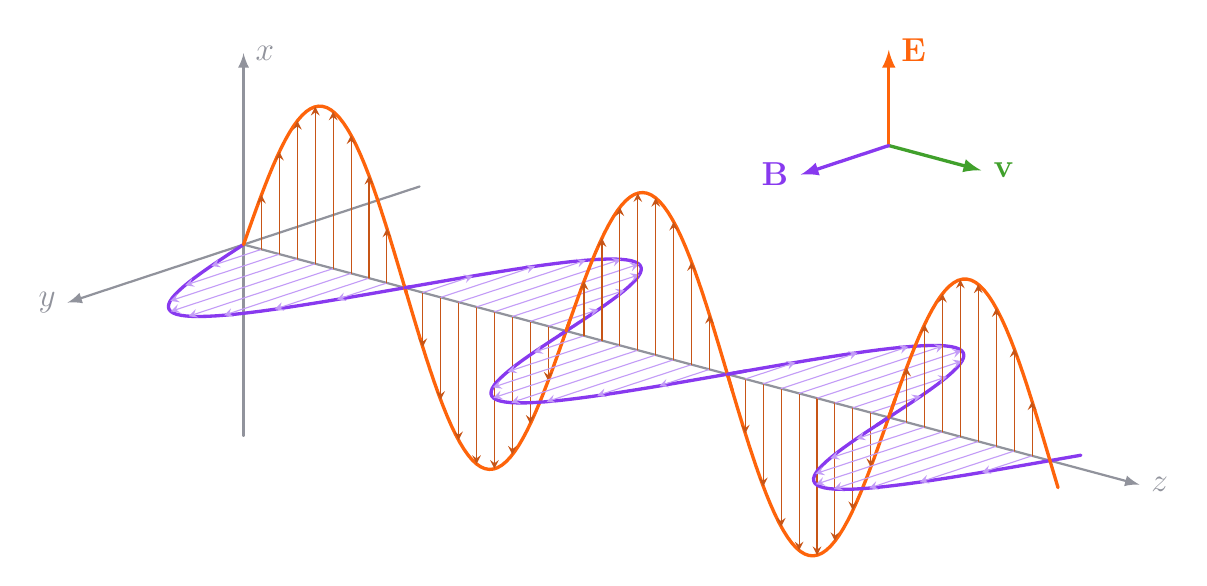
\begin{tikzpicture}[x=(-15:0.9), y=(90:0.9), z=(-150:1.1),
                    line cap=round, line join=round,
                    axis/.style={fg!50!bg, thick,->},
                    vector/.style={>=stealth,->},
                    scale = 1.5]
  \large
  \def\A{1.5}
  \def\nNodes{5} % use even number
  \def\nVectorsPerNode{8}
  \def\N{\nNodes*40}
  \def\xmax{\nNodes*pi/2*1.01}
  \pgfmathsetmacro\nVectors{(\nVectorsPerNode+1)*\nNodes}
  \def\vE{{\color{or}\mathbf{E}}}
  \def\vB{{\color{ma}\mathbf{B}}}
  
  \def\drawENode{ % draw E node and vectors with some offset
    \draw[or,very thick,variable=\t,domain=\iOffset*pi/2:(\iOffset+1)*pi/2*1.01,samples=40]
      plot (\t,{\A*sin(\t*360/pi)},0);
    \foreach \k [evaluate={\t=\k*pi/2/(\nVectorsPerNode+1);
                           \angle=\k*90/(\nVectorsPerNode+1);}]
                in {1,...,\nVectorsPerNode}{
      \draw[vector,or!75!bg]  (\iOffset*pi/2+\t,0,0) -- ++(0,{\A*sin(2*\angle+\iOffset*180)},0);
    }
  }
  \def\drawBNode{ % draw B node and vectors with some offset
    \draw[ma,very thick,variable=\t,domain=\iOffset*pi/2:(\iOffset+1)*pi/2*1.01,samples=40]
      plot (\t,0,{\A*sin(\t*360/pi)});
    \foreach \k [evaluate={\t=\k*pi/2/(\nVectorsPerNode+1);
                           \angle=\k*90/(\nVectorsPerNode+1);}]
                in {1,...,\nVectorsPerNode}{
      \draw[vector,ma!50]  (\iOffset*pi/2+\t,0,0) -- ++(0,0,{\A*sin(2*\angle+\iOffset*180)});
    }
  }
  
  % MAIN AXES
  \draw[axis] (0,0,0) -- ++(\xmax*1.1,0,0) node[right] {$z$};
  \draw[axis] (0,-\A*1.2,0) -- (0,\A*1.2,0) node[right] {$x$};
  \draw[axis] (0,0,-\A*1.2) -- (0,0,\A*1.2) node[left] {$y$};
  
  % SMALL AXES
  \def\xOffset{{(\nNodes-2)*pi/2}}
  \def\yOffset{\A*1.1}
  \def\zOffset{\A*1.1}
  \draw[axis,very thick,gr] (\xOffset,\yOffset,-\zOffset) -- ++(\A*0.6,0,0) node[right,align=center] {$\vb{v}$}; %\\propagation
  \draw[axis,very thick,or]  (\xOffset,\yOffset,-\zOffset) -- ++(0,\A*0.6,0) node[right] {$\vb{E}$};
  \draw[axis,very thick,ma]   (\xOffset,\yOffset,-\zOffset) -- ++(0,0,\A*0.6) node[left] {$\vb{B}$};
  
  % draw (anti-)nodes
  \foreach \iNode [evaluate={\iOffset=\iNode-1;}] in {1,...,\nNodes}{
    \ifodd\iNode \drawBNode \drawENode % E overlaps B
    \else        \drawENode \drawBNode % B overlaps E
    \fi
  }

\end{tikzpicture}
\end{document}
